\documentclass[final]{beamer}

\usepackage[scale=1.2]{beamerposter} % Use the beamerposter package for laying out the poster
\usepackage{caption} % Used to add caption to tabular
%\usepackage{lipsum} % Used for testing purposes
\usepackage{comment}
\usepackage{tcolorbox}
\usepackage[outline]{contour}
\usepackage{amsmath}
\usepackage{amsthm}
\usepackage{amsfonts}
\usepackage{amssymb}
\usepackage{subcaption}
\captionsetup{labelformat=empty}
\usepackage{lipsum}

\definecolor{nibib1}{RGB}{50, 98, 150}
\definecolor{nibib2}{RGB}{57, 160, 237}
\definecolor{nibib3}{RGB}{100, 101, 105}
\definecolor{background}{RGB}{248, 248, 250}
\definecolor{umd}{RGB}{182, 19, 44}

\definecolor{decoder}{HTML}{97CAFF}
\definecolor{encoder}{HTML}{FFD28E}

\makeatletter
\def\thickhline{%
  \noalign{\ifnum0=`}\fi\hrule \@height \thickarrayrulewidth \futurelet
   \reserved@a\@xthickhline}
\def\@xthickhline{\ifx\reserved@a\thickhline
               \vskip\doublerulesep
               \vskip-\thickarrayrulewidth
             \fi
      \ifnum0=`{\fi}}
\makeatother

\newlength{\thickarrayrulewidth}
\setlength{\thickarrayrulewidth}{2\arrayrulewidth}

\usetheme{confposter} % Use the confposter theme supplied with this template

\tcbset{
	colback=white,
    colframe=nibib3,
    coltext=black!80,
    coltitle=gray!5,
    fonttitle=\Large\bfseries,
    center title,
    boxsep=10pt
}

% Many more colors are available for use in beamerthemeconfposter.sty

%-----------------------------------------------------------
% Define the column widths and overall poster size
% To set effective sepwid, onecolwid and twocolwid values, first choose how many columns you want and how much separation you want between columns
% In this template, the separation width chosen is 0.024 of the paper width and a 4-column layout
% onecolwid should therefore be (1-(# of columns+1)*sepwid)/# of columns e.g. (1-(4+1)*0.024)/4 = 0.22
% Set twocolwid to be (2*onecolwid)+sepwid = 0.464
% Set threecolwid to be (3*onecolwid)+2*sepwid = 0.708

\newlength{\sepwid}
\newlength{\onecolwid}
\newlength{\twocolwid}
\newlength{\threecolwid}
\setlength{\paperwidth}{48in} % A0 width: 46.8in
\setlength{\paperheight}{35in} % A0 height: 33.1in
\setlength{\sepwid}{0.012\paperwidth} % Separation width (white space) between columns
\setlength{\onecolwid}{0.235\paperwidth} % Width of one column
\setlength{\twocolwid}{0.482\paperwidth} % Width of two columns
\setlength{\threecolwid}{0.684\paperwidth} % Width of three columns
\setlength{\topmargin}{-0.5in} % Reduce the top margin size
%-----------------------------------------------------------

\usepackage{graphicx}  % Required for including images

\usepackage{booktabs} % Top and bottom rules for tables

\renewcommand{\emph}[1]{{\color{nibib2} #1}}

\setbeamerfont{caption}{size=\footnotesize}

\setbeamercolor{headline}{bg=background}
\setbeamercolor{background canvas}{bg=background}
\setbeamercolor{itemize item}{fg=nibib1,bg=nibib1}

\usepackage{hyperref}
\hypersetup{
    colorlinks=true,
    linkcolor=blue,
    filecolor=magenta,      
    urlcolor=cyan,
}
% 
%----------------------------------------------------------------------------------------
%	TITLE SECTION 
%----------------------------------------------------------------------------------------

\title{Dense 3D Semantic Segmentation for Biomedical Electron Microscopy} % Poster title

\author{{Matthew Guay (matthew.guay@nih.gov),} {Zeyad Emam,} {Adam Anderson,} {Maria Aronova,} {Richard Leapman (leapmanr@mail.nih.gov)}}%\\ ${}^*$} % Author(s)

\institute{\textbf{Laboratory of Cellular Imaging and Macromolecular Biophysics, NIBIB, NIH}} % Institution(s)


%----------------------------------------------------------------------------------------
\setbeamertemplate{headline}{
%  \leavevmode
  \begin{columns}
   \begin{column}{.08\linewidth}
   
\includegraphics[width=1.5\linewidth]{fig/nibiblogo.pdf} 
   \end{column}
   \begin{column}{.84\linewidth}
    \vskip1cm
    \centering
    \usebeamercolor{title in headline}{\color{nibib1}\huge{\textbf{\inserttitle}}\\[0.35ex]}
    \usebeamercolor{title in headline}{\color{umd}\large{\textbf{Board of Scientific Counselors Review}}\\[0.35ex]}
    \usebeamercolor{author in headline}{\color{fg}\large{\insertauthor}\\[1ex]}
    \usebeamercolor{institute in headline}{\color{fg}\large{\insertinstitute}\\[1ex]}
    \vskip1cm
   \end{column}
   \begin{column}{.08\linewidth}
   \hspace{-4.9cm}
%   
\includegraphics[width=1.5\linewidth]{fig/umdlogo.pdf}
   \end{column}
  \end{columns}
 %\vspace{0.2in}
 \hfill\begin{beamercolorbox}[wd=\paperwidth,ht=0.1in]{cboxb}\end{beamercolorbox}\hfill
 %\vspace{0.1in}
}

\addtobeamertemplate{block end}{}{\vspace*{2ex}} % White space under blocks
\addtobeamertemplate{block alerted end}{}{\vspace*{2ex}} % White space under highlighted (alert) blocks


\setlength{\belowcaptionskip}{-0.5ex} % White space under figures
\setlength\belowdisplayshortskip{2ex} % White space under equations

%------------------------------------------------------------------------------------------
\begin{document}

\begin{frame}[t] % The whole poster is enclosed in one beamer frame

\begin{columns}[t] % The whole poster consists of four columns

\begin{column}{\sepwid}\end{column} % Empty spacer column


% First column
\begin{column}{\onecolwid}

    \begin{tcolorbox}[title=Introduction]
        \begin{itemize}
            \item Biomedicine uses \emph{electron microscopy} (EM) to study biological matter at the nanoscale.
            \item Serial block-face scanning electron microscopy (\emph{SBF-SEM}): Image up to $1\,\text{mm}^3$ biological samples at $\sim 5\times 5\times 25\,\text{nm}$ resolution - giga/teravoxel datasets possible.
            \item \emph{Systems biology} will greatly benefit from high-throughput EM, but data analysis is challenging.
            \item \emph{Dense semantic segmentation}: Create rich 3D structural models of all (most) cells and organelles in sample, as opposed to just parts.            
            \item Challenging for computers, slow and challenging for humans.
            \item \emph{Computer vision} (CV) algorithms use neural nets to predict segmentations from 3D image volumes.
 %\emph{Instance} segmentation: Assign a unique tag to each object in an image. %the partitioning of an image into labeled regions corresponding to image content.
            
        \end{itemize}
    \end{tcolorbox}
    
    \begin{center}
        \begin{figure}
            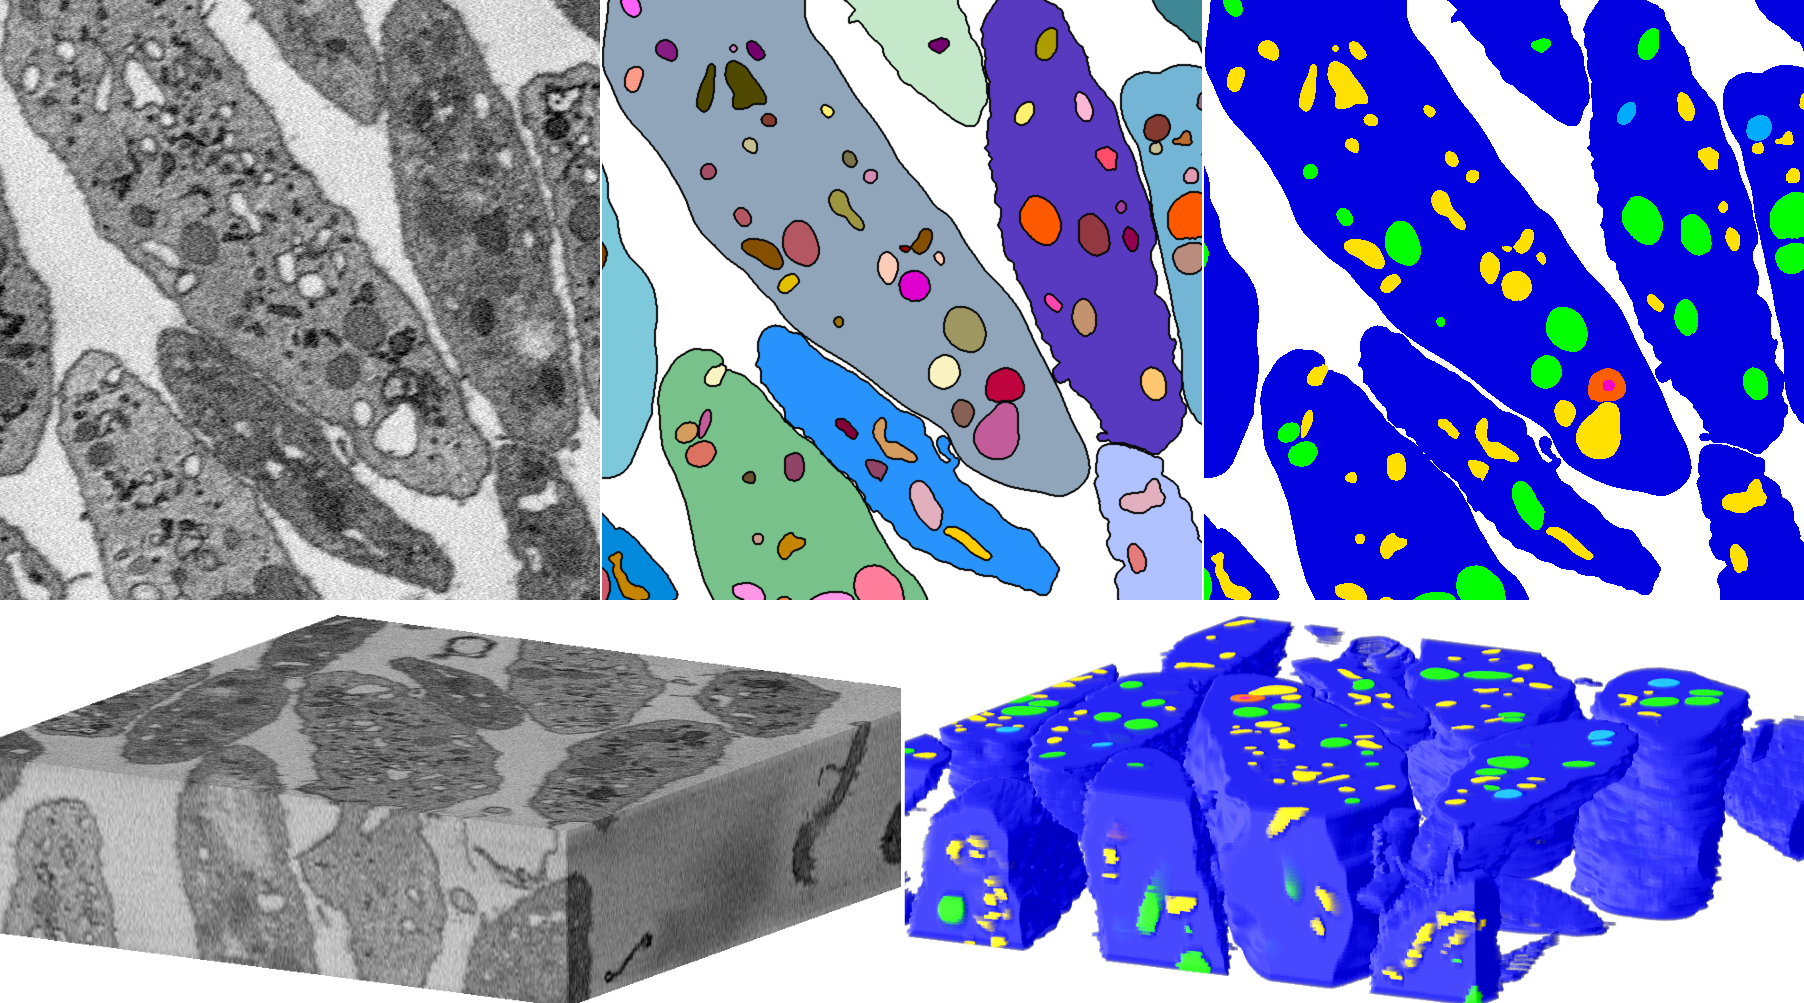
\includegraphics[width=\linewidth]{fig/intronew.png}
            \caption{2D and 3D views of an SBF-SEM platelet dataset and a semantic model of its cells and organelles.}
        \end{figure}
    \end{center}
    
    \begin{tcolorbox}[title=Challenges]
        \begin{itemize}
            \item Training \emph{label generation} is tedious, and experts may disagree.
            \item Lack of \emph{3D benchmark datasets} makes it hard to compare and share tools for biomedical computer vision.  %Different EM hardware + sample combinations create \emph{many image types}.
            \item Automated segmentation is still \emph{not accurate enough} for dense semantic segmentation of interesting biological EM datasets.
            \item \textbf{Goal}: Better \emph{neural architectures} for more useful CV algorithms. 
            \item \textbf{Goal}: Better \emph{software infrastructure} to turn CV algorithms into useful tools for microscopists.
            \item \textbf{Goal}: Release high-quality \emph{3D benchmark datasets} to spur community development.
        \end{itemize}
    \end{tcolorbox}

\end{column} 
% End of first column


\begin{column}{\sepwid}\end{column} % Empty spacer column


% Second column
\begin{column}{\twocolwid}

    \begin{center}
        \begin{figure}
            \includegraphics[width=\linewidth]{fig/result_imgs.png}
            \caption{In the course of this project, we tested many configurations of 2D and 3D segmentation networks and ensembles. This figure shows results from the best 2D and 3D individual networks and ensembles. (\textbf{Top}) Comparison of 2D segmentation cross-sections on the evaluation dataset. (\textbf{Bottom}) Comparison of 3D renderings on one of the test cells from another platelet sample than the one used for training. Testing networks on the same tissue system but a different physical sample helps gauge how robust they are to image variations.}
        \end{figure}
    \end{center}
    
    
    % \begin{tcolorbox}[title=Network Architecture Design]
    %     \begin{itemize}
    %         \item Segmentation networks use combinations of \emph{multi-scale convolutional} modules.
    %         \item Common modules: pooled convolution blocks, dilated convolution blocks, encoder-decoders, spatial pyramid pooling units, more.
    %         \item \emph{Architecture design}: Construction of a computation graph which contains the variables trained during learning.
    %         \item Segmentation network architecture design is a combinatorial search with a \emph{large state space} and \emph{expensive evaluations}.
    %         % \item Module design decisions are represented as numeric \emph{hyperparameters}. 
    %         % \item Simplifies manual and \emph{algorithmic network design}.
    %         % \item Easily generate networks using \emph{multi-level} random hyperparameter sampling.
    %     \end{itemize}
    % \end{tcolorbox}
    
    \begin{columns}[t]
        
    
    \begin{column}{\onecolwid}
        \begin{tcolorbox}[title=Methods]
            \begin{itemize}
                % \item \emph{2D vs 3D} tradeoffs: spatial context vs. memory usage, dealing with anisotropy along $z$ axis.
                \item \emph{Data}: Two SBF-SEM platelet volumes with 6 label classes: Cell, mitochondrion, alpha granule, canalicular system, dense granule, dense core.
                \item \emph{2D-3D network}: Large 2D segmentation module forms intermediate predictions which are input to a smaller 3D segmentation module. Memory efficient, better observed results than 3D alone.
                \item Run architecture generation experiments on \emph{Biowulf} to compare net design choices.
                %\item \emph{Compare against existing baselines} combined with \emph{ablation analyses} to show we outperform the literature with \emph{$2D-3D + 3\times 3\times 3$ nets}.
                %\item A 3D \emph{CRF-RNN} (conditional random field as recurrent neural network) module can be used as well.
                %\item Hybrid-3D + CRF-RNN architecture is currently the best performer.
                % \item \emph{Goal}: Segment a platelet EM image into constituent cells and organelles (mitochondria, canalicular system, alpha granules, dense granules).
                % \item Lab members manually segment a $50\times 800\times 800$ platelet volume for \emph{training data}.
                % \item Train and evaluate 80 random encoder-decoder networks over 24 hours using \emph{Biowulf}, the NIH's HPC system. Compare with the original (Ronneberger et al., 2015) u-net.
                % \item Form \emph{$N$-best} ensembles from the $N$ best networks, determine optimal $N$.
                % \item Segment \emph{new data} using the best ensemble.
                % \item Lab members \emph{correct} network output.
                % \item Goal is \emph{workflow acceleration}, so compare correction time with manual segmentation time.
            \end{itemize}
        \end{tcolorbox}
    \begin{center}
        \begin{figure}
        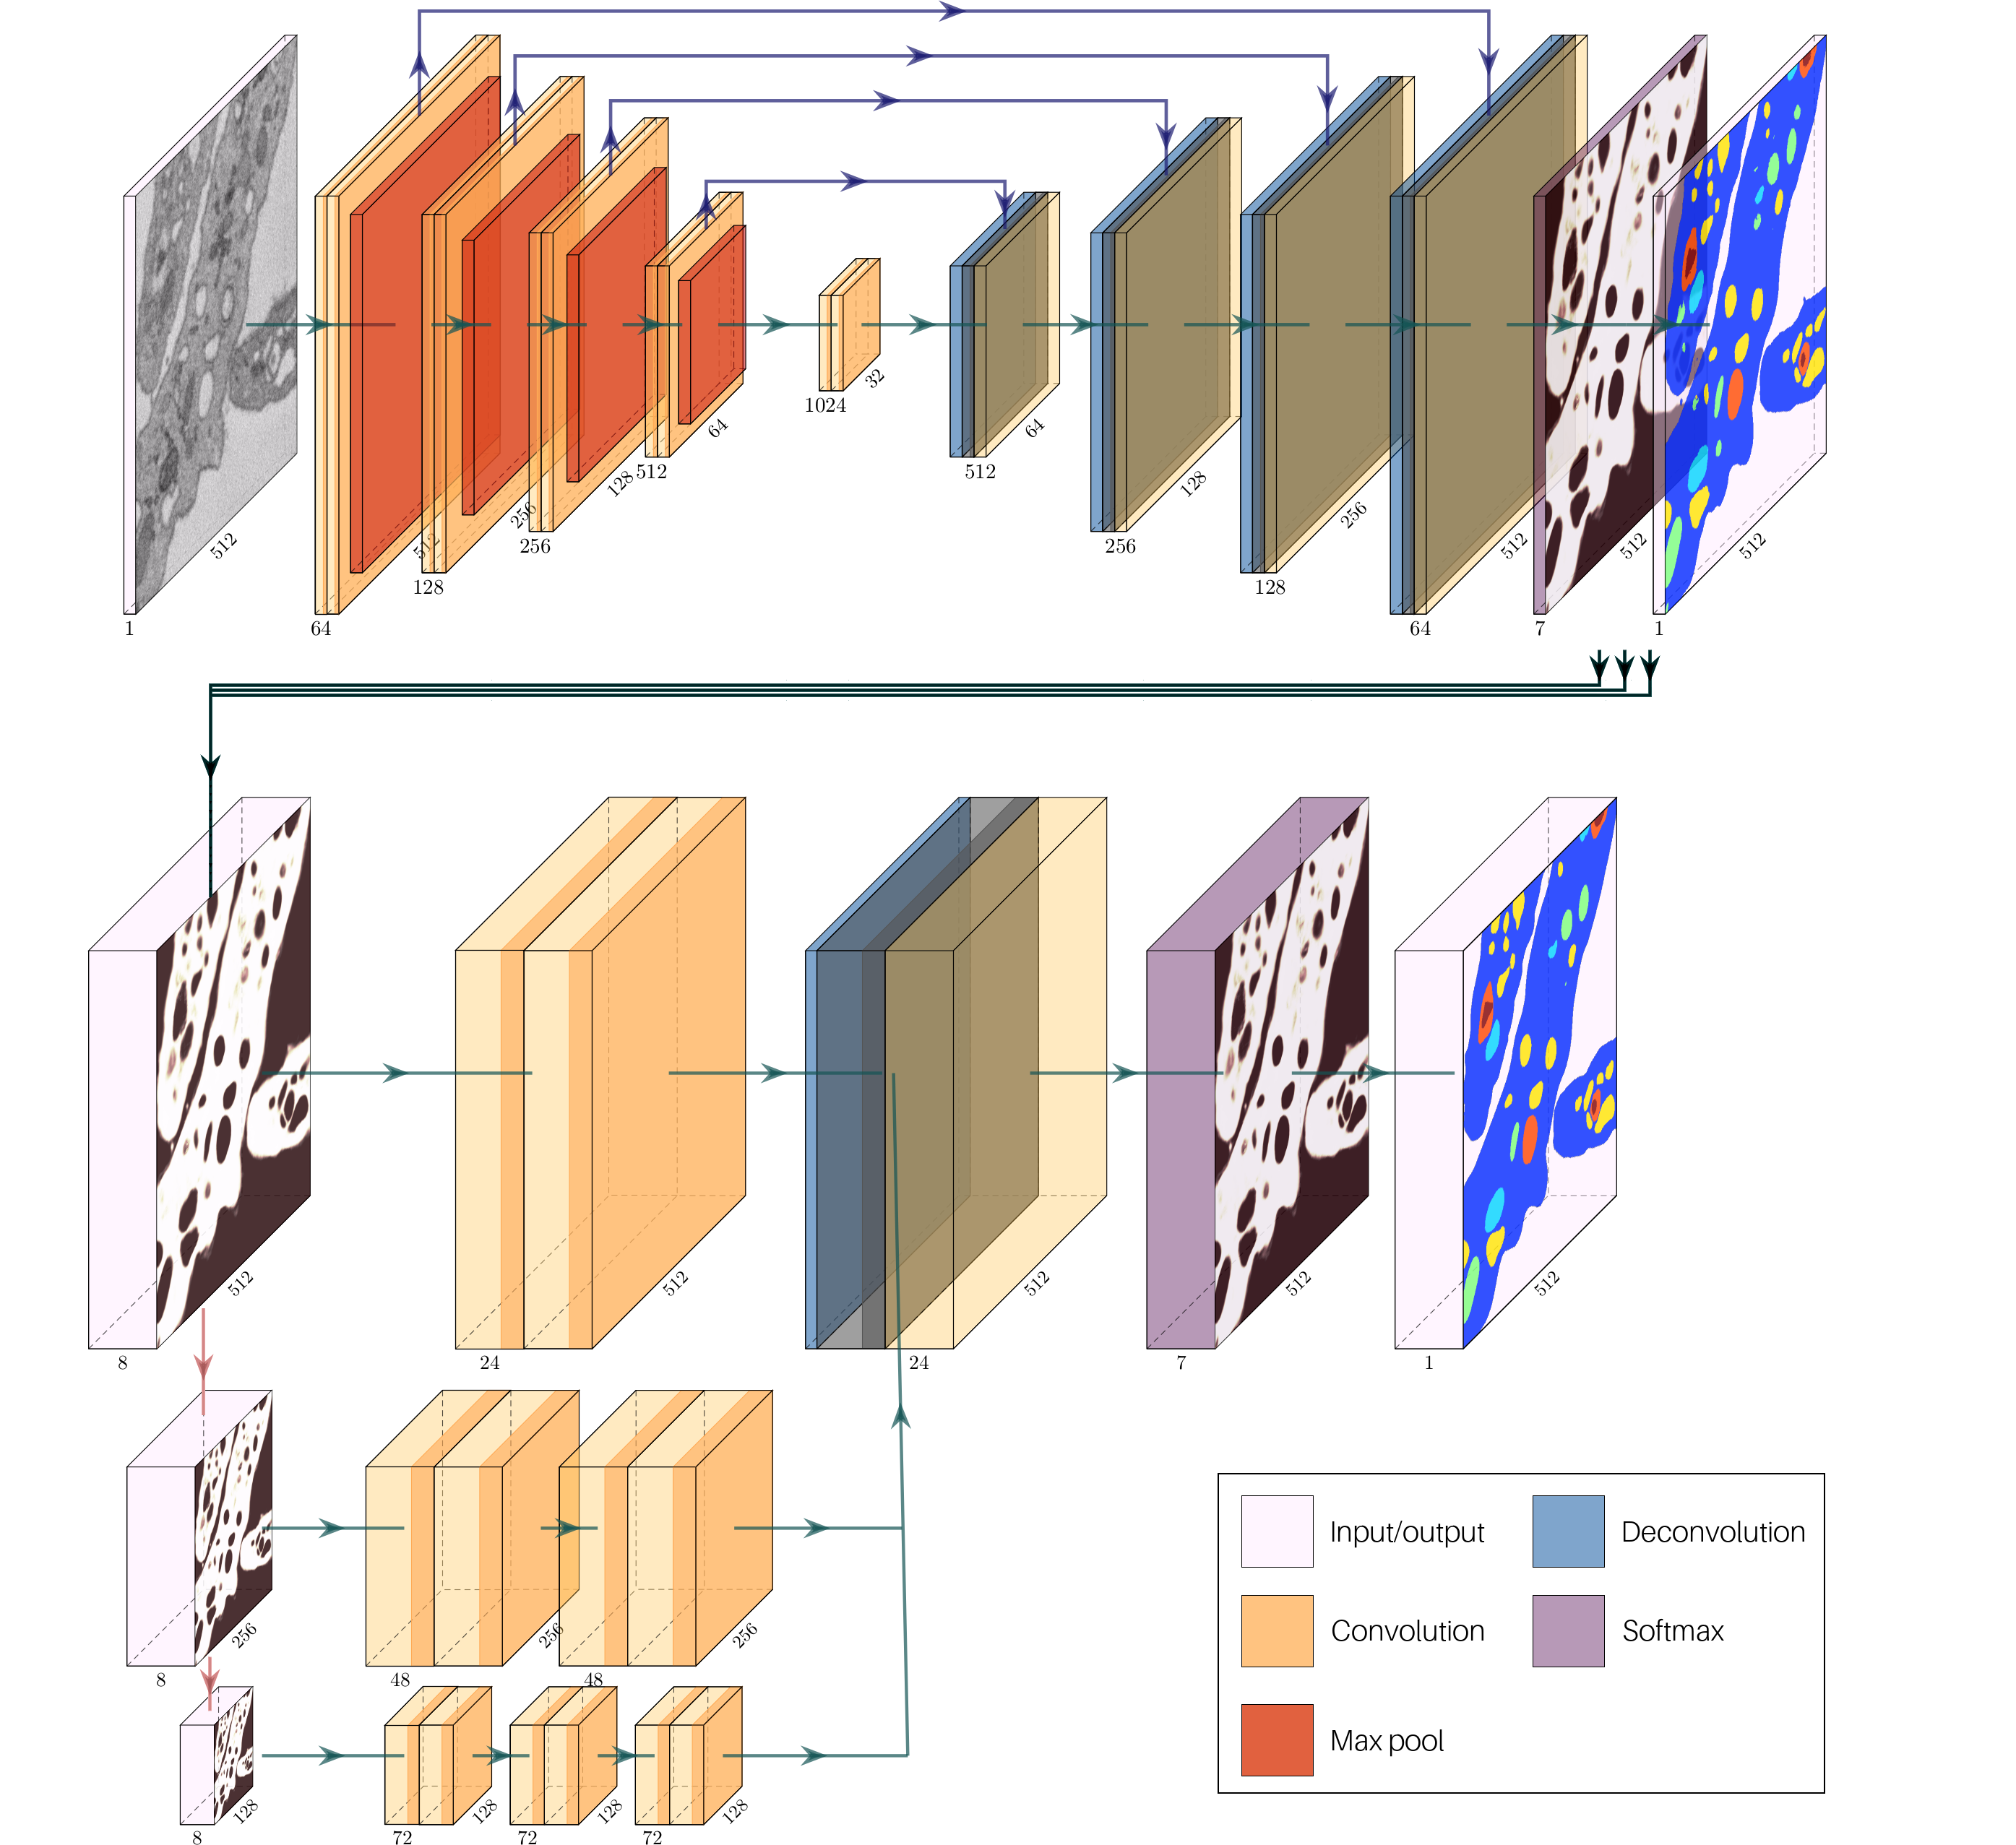
\includegraphics[width=\linewidth]{fig/fullnet-rearranged.png}
        \caption{Diagram of a typical 2D-3D network. A 2D (+3x3x3) encoder-decoder feeds class probabilities from successive 2D image windows into a 3D spatial pyramid module to produce a final segmentation prediction.}
        \end{figure}
    \end{center}
    \end{column}
    \begin{column}{\onecolwid}
    	\begin{tcolorbox}[title=Results]
    	\begin{itemize}
    	\item Overall, a \emph{2D-3D+3x3x3} ensemble performs best on the test dataset, the best indicator of generalization ability. 
    	\item 3x3x3 ablation better on eval. Difference is not significant compared with same-net variations between training sessions.
    	\item 3D nets better than 2D nets. Ensembles better than individual nets.
    	\item All LCIMB nets perform much better than existing baselines like DeeplabV3, DeepVess, and MedicalNet when trained on our segmentation task.
    	\end{itemize}
    	\end{tcolorbox}
    	
    	\bgroup
\begin{table}
\centering
\def\arraystretch{1.2}
\begin{tabular}{l l l}
\thickhline
Architecture & Eval MIOU & Test oMIOU\\
\hline
Ens. 2D-3D+3x3x3 4 & 0.686 & \textbf{0.553} \\
Ens. Abl. 3x3x3 Convs 5 & \textbf{0.690} & 0.520 \\
\hline
Ens. 2D-3D 4 & 0.688 & 0.470 \\
2D-3D+3x3x3 & 0.665 & 0.547 \\
2D-3D & 0.650 & 0.477 \\
Abl. 3x3x3 Convs & 0.667 & 0.466 \\
Abl. Multi-Loss & 0.652 & 0.467 \\
Abl. 3D Pyramid & 0.646 & 0.487 \\
Ens. Abl. Multi-Loss 3 & 0.633 & 0.445 \\
Ens. Abl. 3D Pyramid 3 & 0.681 & 0.533 \\
\thickhline
\end{tabular}
\caption{3D network results summary. Mean intersection-over-union (MIOU) on eval data and organelle MIOU (oMIOU) on test data. 2D experiments and baselines not shown. \textit{Abl.} short for ablation, \textit{Ens.} short for ensemble. The test dataset contains only a small number of labeled cells among unlabeled ones; restricting the MIOU stat to the labeled region invalidates \texttt{cell} class statistics, hence the use of oMIOU.}
\end{table}
\egroup
    \end{column}
    
    \end{columns}

\end{column}
% End of second column


%\begin{column}{\sepwid}\end{column} % Empty spacer column


% Third column
% \begin{column}{\onecolwid}


% \begin{tcolorbox}[title=Modular Network Generation]
% \begin{itemize}
% \item \emph{Algorithmic} architecture design: automatically search the architecture design space.
% %\item Observation: Segmentation networks form hierarchical \emph{module trees}: A tree of modules built up from repeated, simpler modules.
% \item \emph{Random sampling} of module hierarchy trees finds effective segmentation architectures with modest computational resources.
% %\item Combine with other \emph{black box optimization} tools to improve parameters that do not alter the module hierarchy.
% \item Run architecture search on NIH's \emph{Biowulf} using new distributed evaluation tools. Combining best nets into \emph{ensembles} for improved prediction.
% \end{itemize}
% \end{tcolorbox}
% \vspace{.1in}


% End of third column


\begin{column}{\sepwid}\end{column} % Empty spacer column


% Fourth column
\begin{column}{\onecolwid}
    
    \begin{tcolorbox}[title=Future Work]
		\begin{itemize}
            \item \emph{Robust segmentation}: Train a single segmentation model that works across multiple datasets. May involve:
            \begin{itemize}
            \item Transfer learning of networks or network modules between datasets.
            \item \emph{Hierarchical semantics}: Predict a hierarchy of both broad and narrow classes to better deal with unknown structures.
            \end{itemize}
            \item \emph{Panoptic segmentation} for biological EM: Combining semantic and instance segmentation to generate 3D object meshes and semantics from images.
            \item \emph{Expand benchmark dataset}: Currently assembling a collection of annotated EM image volumes for release to the machine learning community: \href{https://bio3d-vision.github.io/}{https://bio3d-vision.github.io/}.
            \item Use a \emph{correction-training feedback loop} to produce large amounts of labeled training data. Requires integrating machine learning tools with established in-lab analysis software.
            \item \emph{Active learning:} Develop algorithms to determine which data is most \textit{informative}. 
            \item \emph{Intramural collaboration} to build a biological microscopy scientific computing + machine learning team with the size necessary to address research and applications in their full scope.
        \end{itemize}
    \end{tcolorbox}
    
    \begin{tcolorbox}[title=References]
        \nocite{GuayDesigning2018}
        \nocite{Guay2018problems}
        \bibliographystyle{ieeetr}
        \bibliography{bib}
        
    \end{tcolorbox}

    \begin{tcolorbox}[title=Acknowledgements]
        \begin{itemize}
            \item This work made use of the computational resources of the \emph{NIH HPC Biowulf cluster}.
            \item Data for this project was acquired in collaboration with Professor Brian Storrie's lab at UAMS (\href{https://physiology.uams.edu/faculty/brian-storrie/}{link}).            
            \item \emph{View this poster online} at \href{https://leapmanlab.github.io/bsc-2019/poster.pdf}{https://leapmanlab.github.io/bsc-2019/poster.pdf}.
        \end{itemize}
    \end{tcolorbox}
    
    
\end{column}
% End of fourth column

\end{columns}

\end{frame}

\end{document}

